\section{Background and Related Work} \label{BACK}

In this section, we present the background on Network Functions Virtualization (NFV) and Virtualized Network Function (VNF). We also discuss the characteristics of existing VNF platforms as well as the basic requirements that they must address.

\subsection{Network Function Virtualization in a Nutshell} \label{VISAO}

NFV aims to implement Network Functions (NFs) in software, so they can run on commodity hardware by employing common virtualization technologies \cite{ETSI-2012}. Two of the most relevant standardization bodies are expending considerable energy in defining models, methodologies, and concepts in this area: the European Telecommunications Standards Institute (ETSI) and the Internet Engineering Task Force (IETF).

The NFV architectural framework \cite{GS-2014} defined by ETSI is composed of three functional blocks: NFV Infrastructure (NFVI), NFV Management and Orchestration (NFV MANO), and Virtualized Network Functions (VNF). NFVI is the collection of physical resources (\textit{e.g.}, processing, storage, and network) needed to execute VNFs. NFV MANO in turn encompasses: the Virtualized Infrastructure Manager (VIM), which controls the physical/software infrastructure; the VNF Manager (VNFM), which is responsible for VNF lifecycle operations (\textit{e.g.}, instantiation, termination, scaling, and migrations); and the NFV Orchestrator (NFVO), which enables the management of network services. Finally, the VNF functional block itself represents the network functions that run on VNF platforms.

Because of the development flexibility offered by NFV, advanced network services can be quickly created and deployed, such as NFV-based security solutions (\textit{e.g.}, DeMONS \cite{Garcia-2018}, VFence \cite{Jakaria-2016}, and \cite{Cunha-2018}), \blue{as well as common network services, such as DHCP, DNS and Routing}.

%These sophisticated functions are designed through the composition of multiple VNF Components (VNFC) \cite{GS-2014-2}. Usually, a standalone VNFC performs a specific functionality with lower complexity, but the combination of VNFCs enables the creation of complete VNFs. In general, a VNFC is also a virtualized element, but its lifecycle depends on its parent VNF.

The IETF has been working on standardizing the Service Function Chain (SFC) \cite{Joel-2015}, which consists of multiple VNFs working together in a composition that provides a network service. In addition to internal VNFs, a SFC also includes boundary nodes (\textit{i.e.},  incoming and outgoing points of traffic) and steering specifications. One way to implement those SFCs is by using the architecture defined in the IETF's Request for Comments (RFC) number 7665 \cite{Joel-2015}. In that RFC, a Network Service Header (NSH) \cite{Quinn-2018} is employed to enable packets to traverse a specific path of VNFs. Each VNF, in turn, can either be NSH-aware or not. NSH-aware VNFs make a request to a proxy element to remove the NSH before processing, after which the proxy element is again invoked to update/reinsert the NSH element. Alternatively, VNFs can process NSH themselves, without relying on external elements.

An NSH encapsulates L3 packets as they are processed by the SFC, and carries information about the Service Function Path (SFP), the current packet location in the SFP, and meta-data provided by the VNFs during packet processing.  NSH is subdivided into three meta-headers: Base Header, Service Path Header, and Context Header. The Base Header provides general information about the protocol itself and the next meta-headers data. This meta-header (4 bytes), in turn, carries 5 fields (\textit{i.e.}, version, O bit, TTL, length, and meta-data type), in addition to reserved space for future protocol use. The Service Path Header is also formed by 4 bytes and has 2 fields: Service Path Identifier (identifies the SFC's SFP) and the Service Index (provides the location of the packet in the SFP). Finally, the Context Header can be fixed (16 bytes) or variable to carry meta-data information as the SFC is processed. NSH is depicted in Figure \ref{FIG:NSH}.

\begin{figure}[!h]
\centering
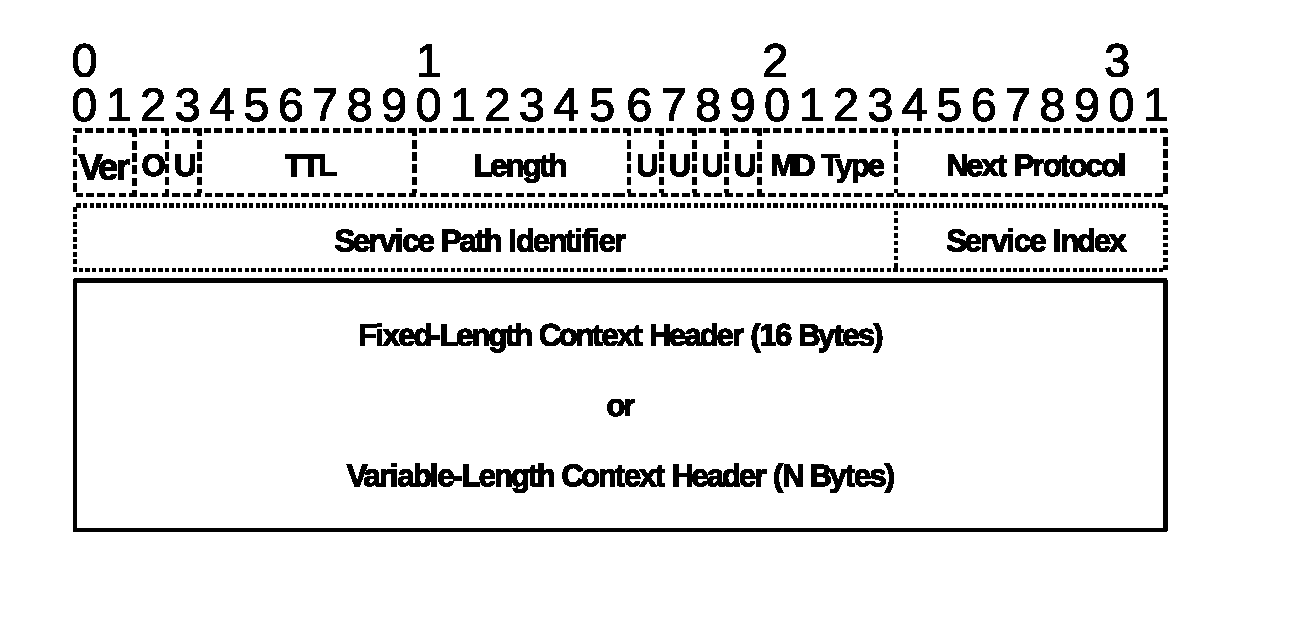
\includegraphics[width=\linewidth]{images/NSH.eps}
\caption{Network Service Header}
\label{FIG:NSH}
\end{figure}

%VNF platforms are specially designed to host VNFs and their associated components. The ETSI lists the basic requirements for developing such platforms (\textit{e.g.}, hardware independence, elasticity, reliability) \cite{SWA-2014}. The ETSI also specifies that a VNF platform must host VNFs independently of the underlying hardware. Furthermore, VNF platforms must provide the flexibility expected from the NFV paradigm to support the operations of deployment, scaling, and migration.

VNF platforms are specially designed to host VNFs and their associated components. The ETSI lists the basic requirements for developing such platforms (\textit{e.g.}, hardware independence, elasticity, reliability) \cite{SWA-2014}. The ETSI also specifies that a VNF platform must host VNFs independently of the underlying hardware. Furthermore, VNF platforms must provide the flexibility expected from the NFV paradigm to support the operations of deployment, scaling, and migration.

%The fundamental NFV requirements that must  be fulfilled by VNF platforms in order to support VNF execution, according to the ETSI \cite{ISG-2013}, are:

%\begin{itemize}
%    \item \textbf{Portability} -- VNFs from different vendors should execute independently of platforms and infrastructures employed. Therefore, it is essential to use unified interfaces that isolate the instances of VNFs from the associated physical infrastructure.

%    \item \textbf{Performance} -- The use of NFV-based technologies may lead to performance degradation in comparison with the performance of middleboxes. That happens mostly due to non-optimized network hardware and inadequate software solutions (\textit {i.e.}, without virtualization optimizations).

%    \item \textbf{Integration} -- Network operators must be able to employ multiple physical servers, hypervisors, and VNFs of different technologies without limitations.

%    \item \textbf{Management and Orchestration} -- VNFs should provide adequate management interfaces for both network operators and other functional blocks of the NFV architecture. Examples of Management and Orchestration requirements include easy and efficient VNF configuration, instantiation, provisioning, and design \cite{Bondan-2014}.

%    \item \textbf{Scalability} -- VNFs must be easily scaled, instantiated, and migrated to support the ever-changing needs of network operators.
%\end{itemize}

%Several aspects of VNF platforms, however, are still unexplored in the literature. For example, the lack of standards for the internal modules have led to several solutions, mostly created without integration in mind neither support for well-accepted management models. Existing platforms, detailed next, usually support only a single programming language, run on very specific hypervisors, do not describe a formal architecture, and do not fulfill all the above requirements defined by the ETSI.

Several aspects of VNF platforms, however, are still unexplored in the literature. For example, the lack of standardization on existing VNFs platforms, mostly created without a well defined architecture and missing features such as NSH and SFC support. Existing platforms, detailed next, usually support only a single programming language, run on very specific hypervisors, do not describe a formal architecture, and do not fulfill all the above requirements defined by the ETSI.


\subsection{VNF Platforms} \label{PEVNFS}

Many research efforts concentrate on creating VNF platforms that are capable of executing NFs. However, these VNF platforms do not provide support for more recent NFV specifications, such as NSH. Still, two of the most important VNF platforms today are ClickOS and OpenNetVM, described next.

ClickOS \cite{Martins-2014} is an optimized platform for running NFs based on Mini-OS, \textit{netmap}, and \textit{Click Modular Router}. ClickOS uses paravirtualization techniques along with several modifications in both Xen and VALE to support fast packet I/O, being able to saturate 10GbE links with a single processing core. Alas, the ClickOS architecture is monolithic and inflexible and supports only a single packet acceleration tool for sending and receiving network traffic to an indivisible NF.

OpenNetVM \cite{Zhang-2016} is a simplified platform that uses containers to execute VNFs on commodity servers along with the packet acceleration framework DPDK \cite{Intel-2014}. OpenNetVM meets the ETSI scalability requirements because of its lower overhead due to the use of containers, which are a lightweight solution in comparison with virtual machines. The OpenNetVM architecture consists of a packet acceleration tool interconnecting VNFs with Virtualized NICs (VNICs). NFs are created as a single component within a proprietary framework and are deployed on a container core. OpenNetVM also provides an internal router implemented using shared memory, which steers network traffic between multiple VNFs.

Both ClickOS and OpenNetVM unfortunately lack support for important VNF elements (\textit{e.g.}, VNFCs and NSH). The ClickOS architecture is straightforward and does not have any native management method, providing only a minimalist environment to execute simple NFs. Despite OpenNetVM's internal traffic router, the platform is restricted to a single packet acceleration tool and a single packet processing framework, both deployed on a container core and managed by an external native agent. Furthermore, these platforms do not meet all of the requirements specified by the ETSI. ClickOS, for example, can only be executed on the Xen hypervisor and every control operation is performed locally through the XenStore. Also, OpenNetVM presents limitations related to NF instantiation (due to hardware device sharing), portability (migrations are only possible between compatible infrastructures), and security issues with containers (single kernel sharing) \cite{Manco-2017}.
